\begin{frame}
    \frametitle{Научная новизна}
    \begin{itemize}
        \item Получены новые априорные оценки решений начально-краевых задач для
        квазистационарных и квазилинейных уравнений сложного теплообмена и до
        казана их нелокальная однозначная разрешимость.
        \item Представлены априорные
        оценки решений регуляризованных задач и обоснована сходимость их решений к
        точным решениям обратных задач.
        \item Для решения задач с фазовыми ограничениями,
        предложены алгоритмы, основанные на аппроксимации экстремальными
        задачами со штрафом.
        \item Реализованы программные комплексы
        \begin{enumerate}
            \item По решению обратных задач, основанные на оптимизационных методах
            \item Тестирования решений, получаемых в результате решения обратных задач
            \item Инструменты моделирования процессов сложного теплообмена для манипуляции `in place`
            \item Инструменты визуализации получаемых значений в процессе моделирования
        \end{enumerate}
    \end{itemize}
    \begin{minipage}[t]{.25\linewidth}
        \center{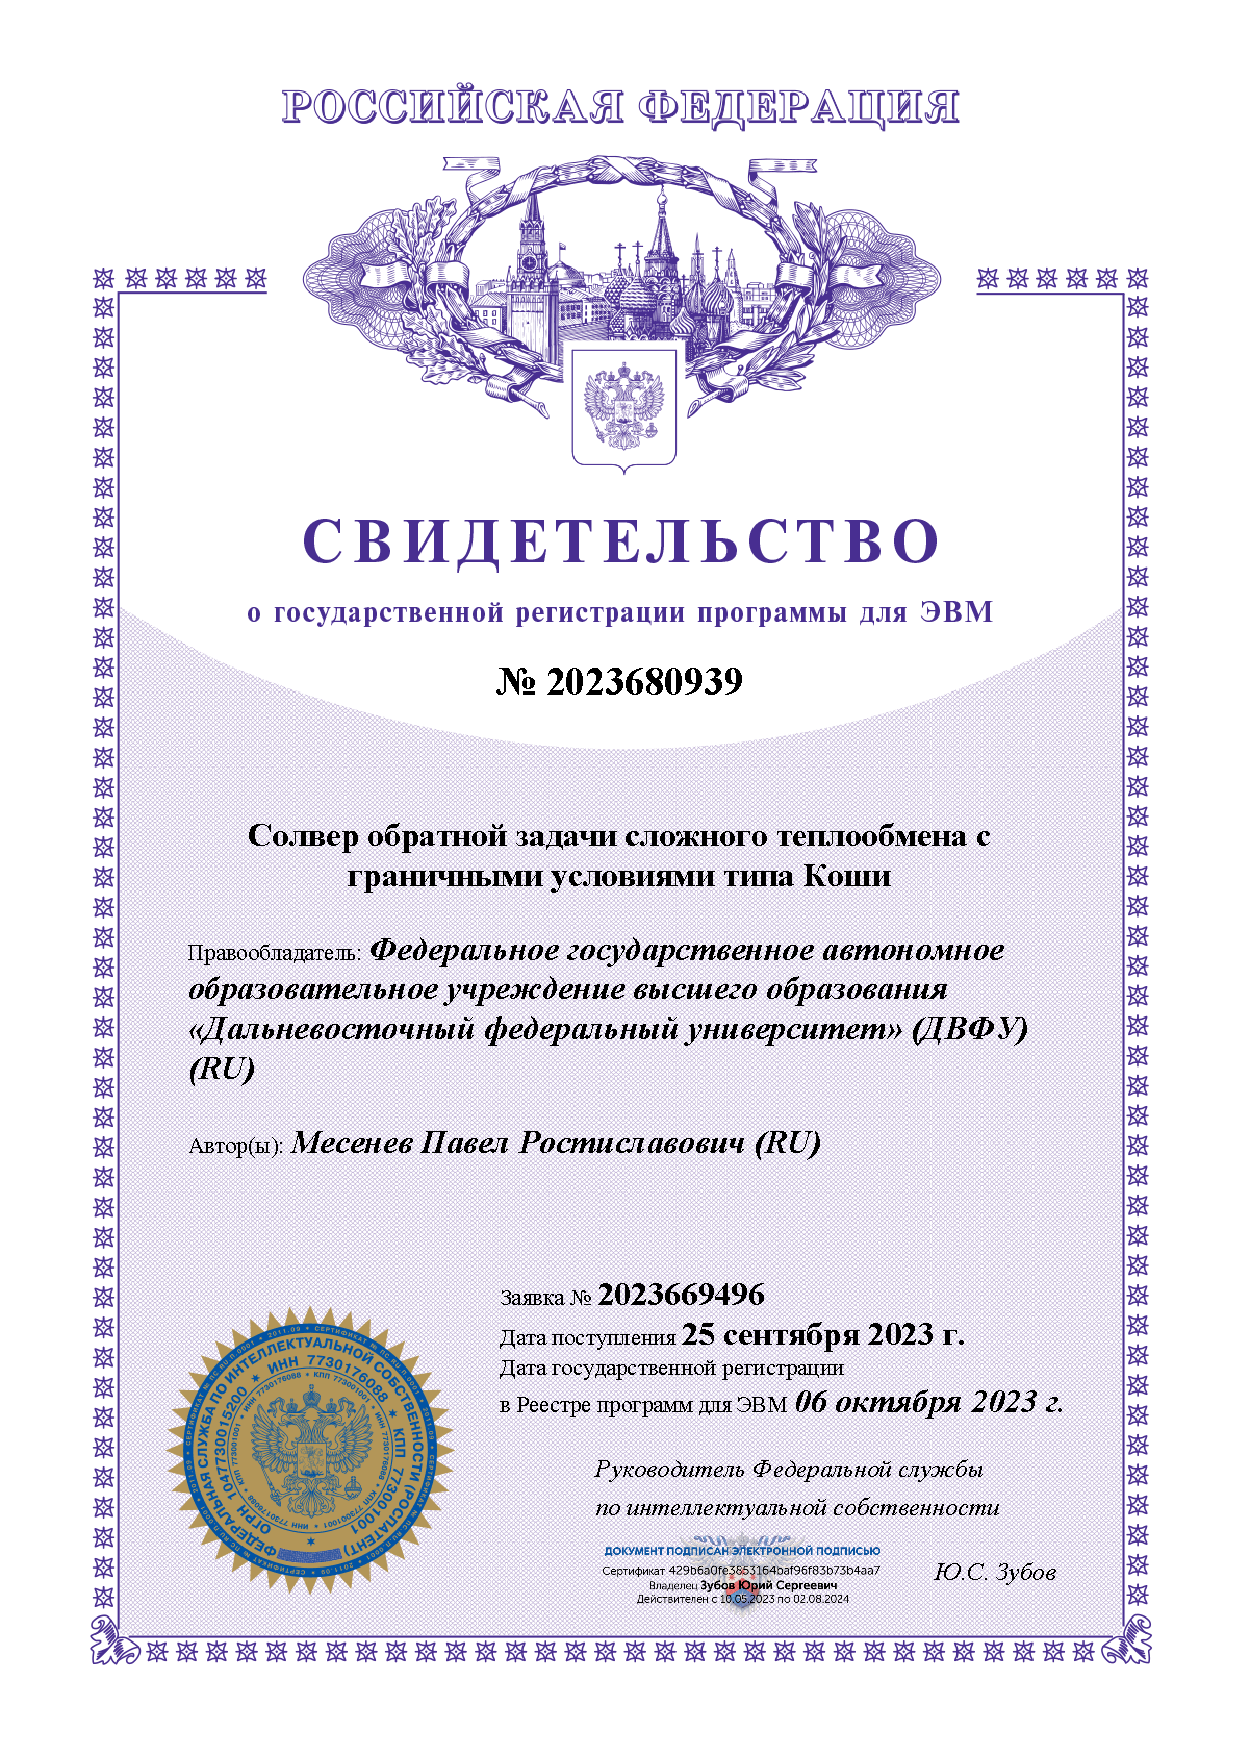
\includegraphics[width=1\linewidth]{reg1}}
    \end{minipage}
    \hfill
    \begin{minipage}[t]{.25\linewidth}
        \center{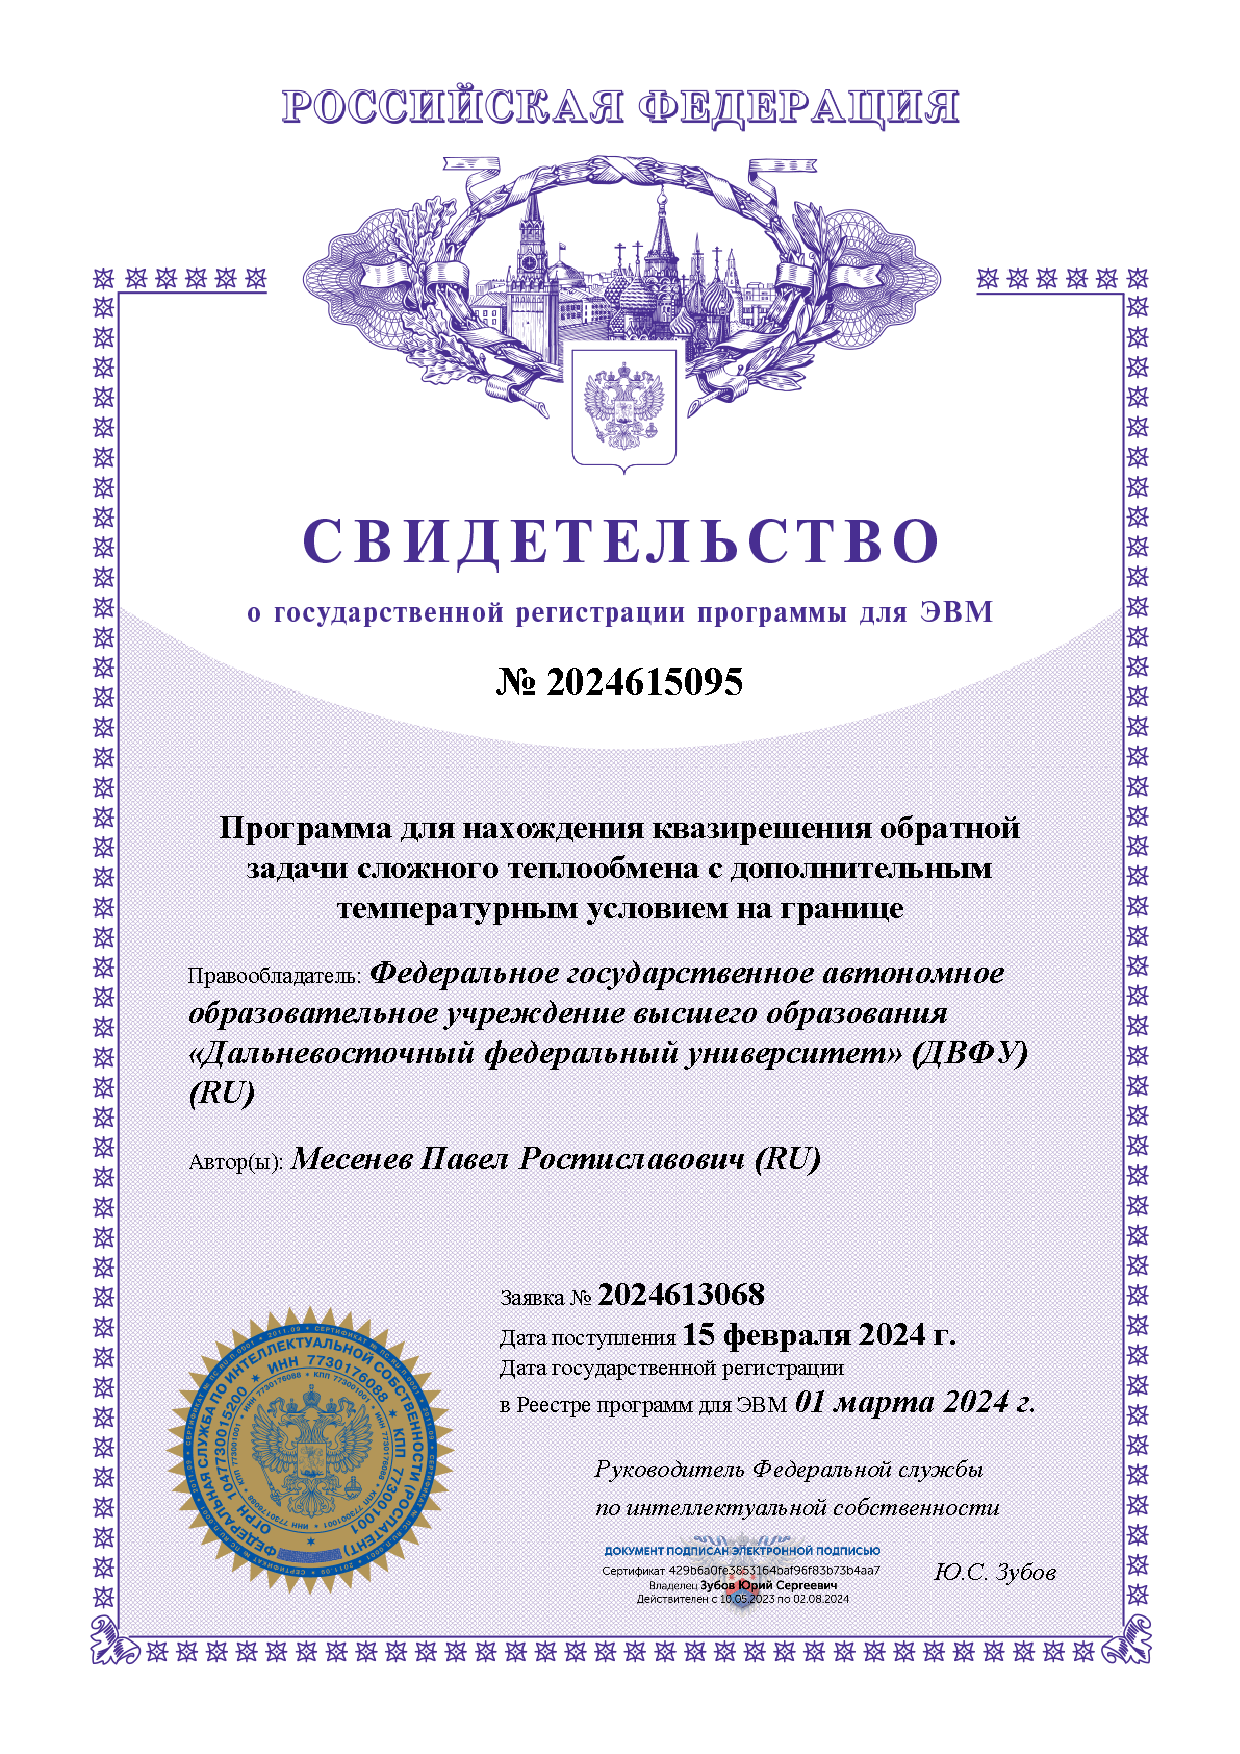
\includegraphics[width=1\linewidth]{reg2}}
    \end{minipage}
    \hfill
    \begin{minipage}[t]{.25\linewidth}
        \center{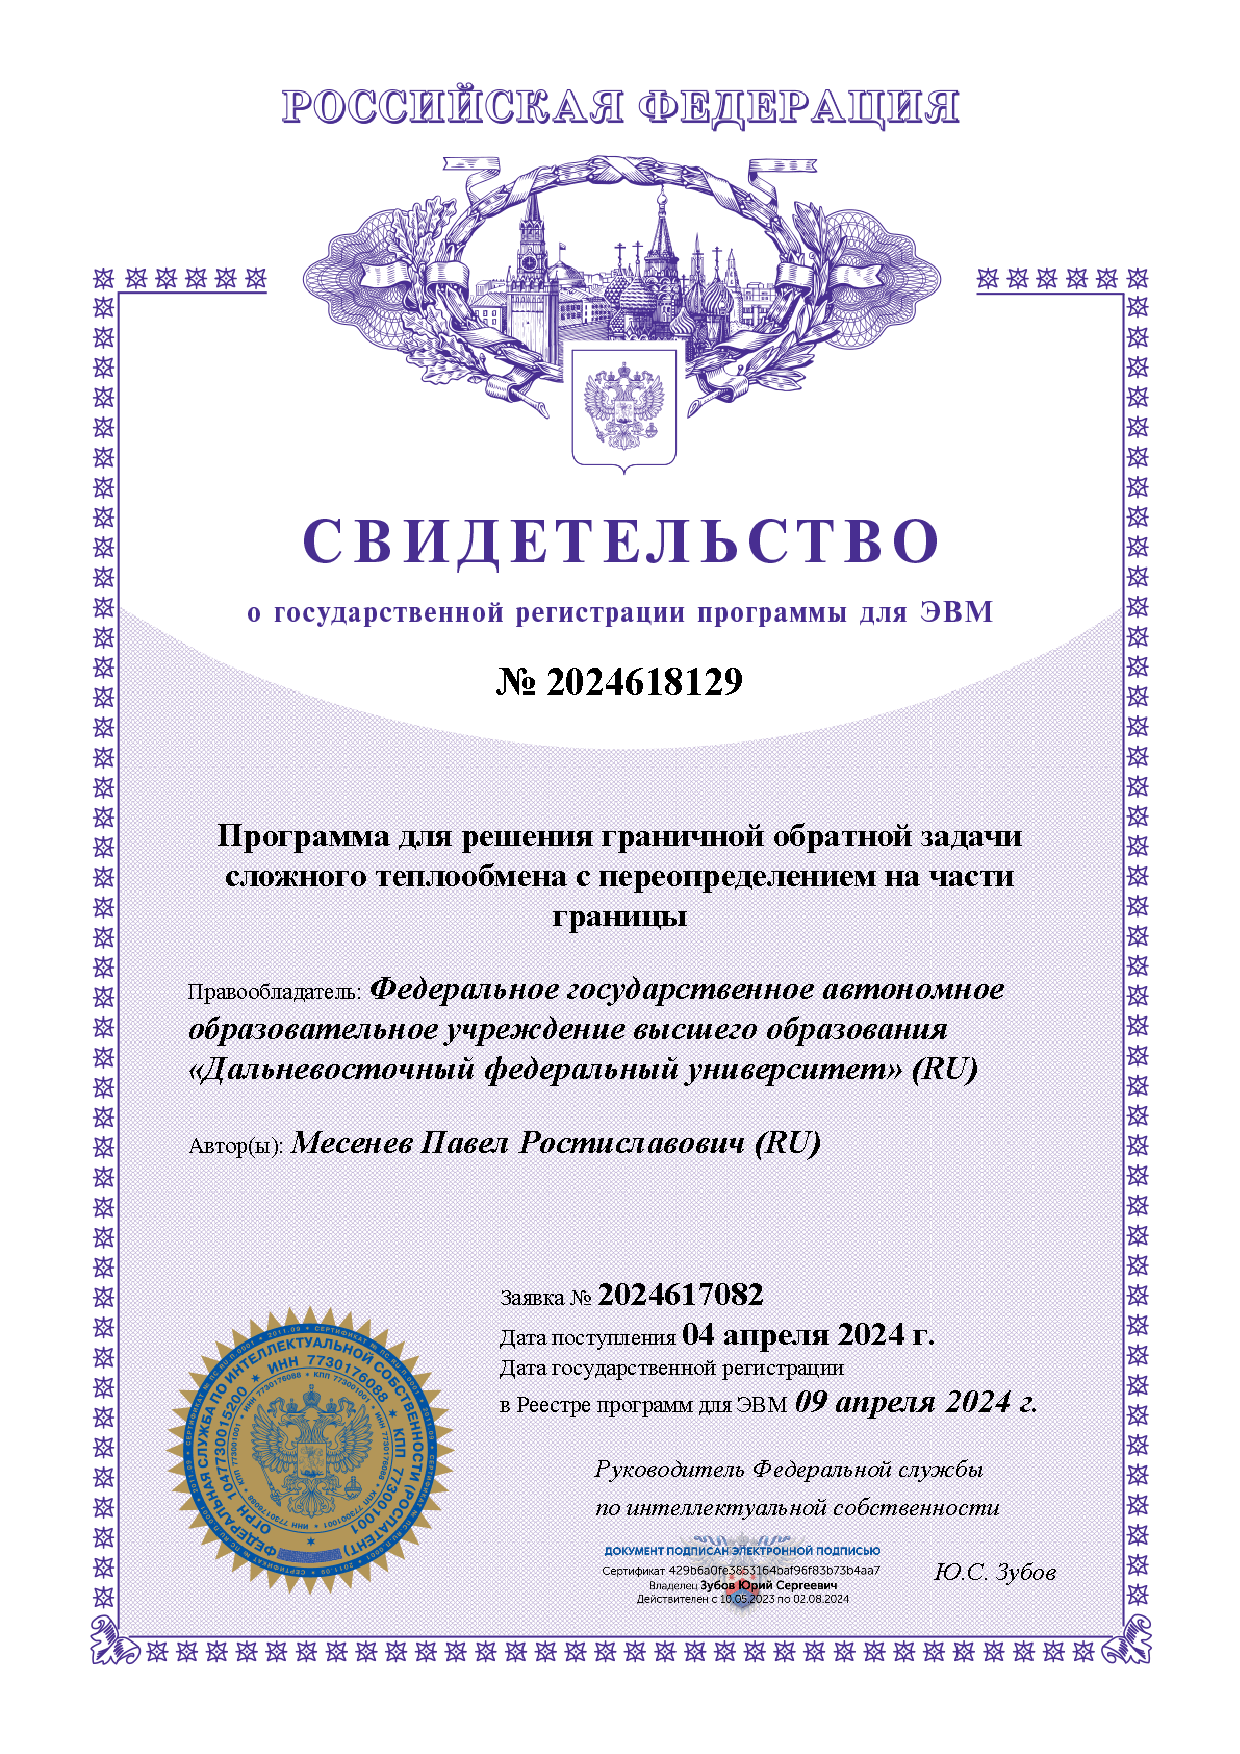
\includegraphics[width=1\linewidth]{reg3}}
    \end{minipage}
\end{frame}



\begin{frame} % публикации на одной странице
    \frametitle{Публикации, конференции}
    ВАК:
    \small{
        \begin{enumerate}
            \item P. R. Mesenev\ — \textit{Дальневост. матем. журн.} 23.1 (2023).

            \item П. Р. Месенев и А. Ю. Чеботарев
            — \textit{Ж. вычисл. матем. и матем. физ.} (2023).

            \item P R Mesenev and A Yu Chebotarev
            — \textit{Comput. Math. Math. Phys. 62.1} (Jan. 2022).

            \item A. Yu. Chebotarev, N. M. Park, P. R. Mesenev и A. E. Kovtanyuk
            — \textit{Dal’nevostochnyi Matematicheskii Zhurnal} (2022).

            \item A. Yu. Chebotarev и P. R. Mesenev
            — \textit{Dal’nevostochnyi Matematicheskii Zhurnal} (2020).

            \item P. R. Mesenev и A. Yu. Chebotarev
            — \textit{Dal’nevostochnyi Matematicheskii Zhurnal} (2018).
        \end{enumerate}
    }
    Прочее:
    \small{
        \begin{enumerate}
            \item A. Chebotarev, A. Kovtanyuk, P. Mesenev
            — \textit{Proceedings
            of the Workshop on Mathematical Modeling and Scientific Computing:
            Focus on Complex Processes and Systems – Dedicated to the Memory of
            Nikolai Botkin} (2020).

            \item A Yu Chebotarev, N M Park, P R Mesenev и A E Kovtanyuk
            — \textit{ Journal of Physics: Conference Series} (2023).

            \item A. Chebotarev, P. Mesenev и A. Kovtanyuk
            — \textit{2023 Days on Diffraction (DD)} (2023).

            \item A. Chebotarev, A. Kovtanyuk, N. Park, P. Mesenev
            — \textit {2021 Days on Diffraction (DD)} (2021).

            \item П. Р. Месенев
            — \textit{Материалы региональной научно-практической
            \item конференции студентов, аспирантов и молодых учёных по
            естественным наукам} (2018)
        \end{enumerate}
    }

    Конференции:
    \small{
        \begin{itemize}
            \item Региональная научно-практическая конференция (Владивосток, 2018, 2019);
            \item Workshop on Computing Technologies and Applied Mathematics (Владивосток, 2022);
            \item Int.\ Conference DAYS on DIFFRACTION (Санкт-Петербург, 2021, 2023);
            \item Int.\ Workshop on Math.\ Modeling and Scientific Computing (Мюнхен, 2020, 2022).
        \end{itemize}
    }
\end{frame}
